\chapter{Planeación del proyecto}

\section{Estructura de trabajo}

El proyecto se divide en siete paquetes: alcance, investigación, subneteo, arquitectura, automatización, pruebas y entrega. Cada paquete produce un artefacto revisable. La documentación se desarrolla junto con la infraestructura para evitar reconstruir decisiones al final.

\begin{figure}[H]
\centering
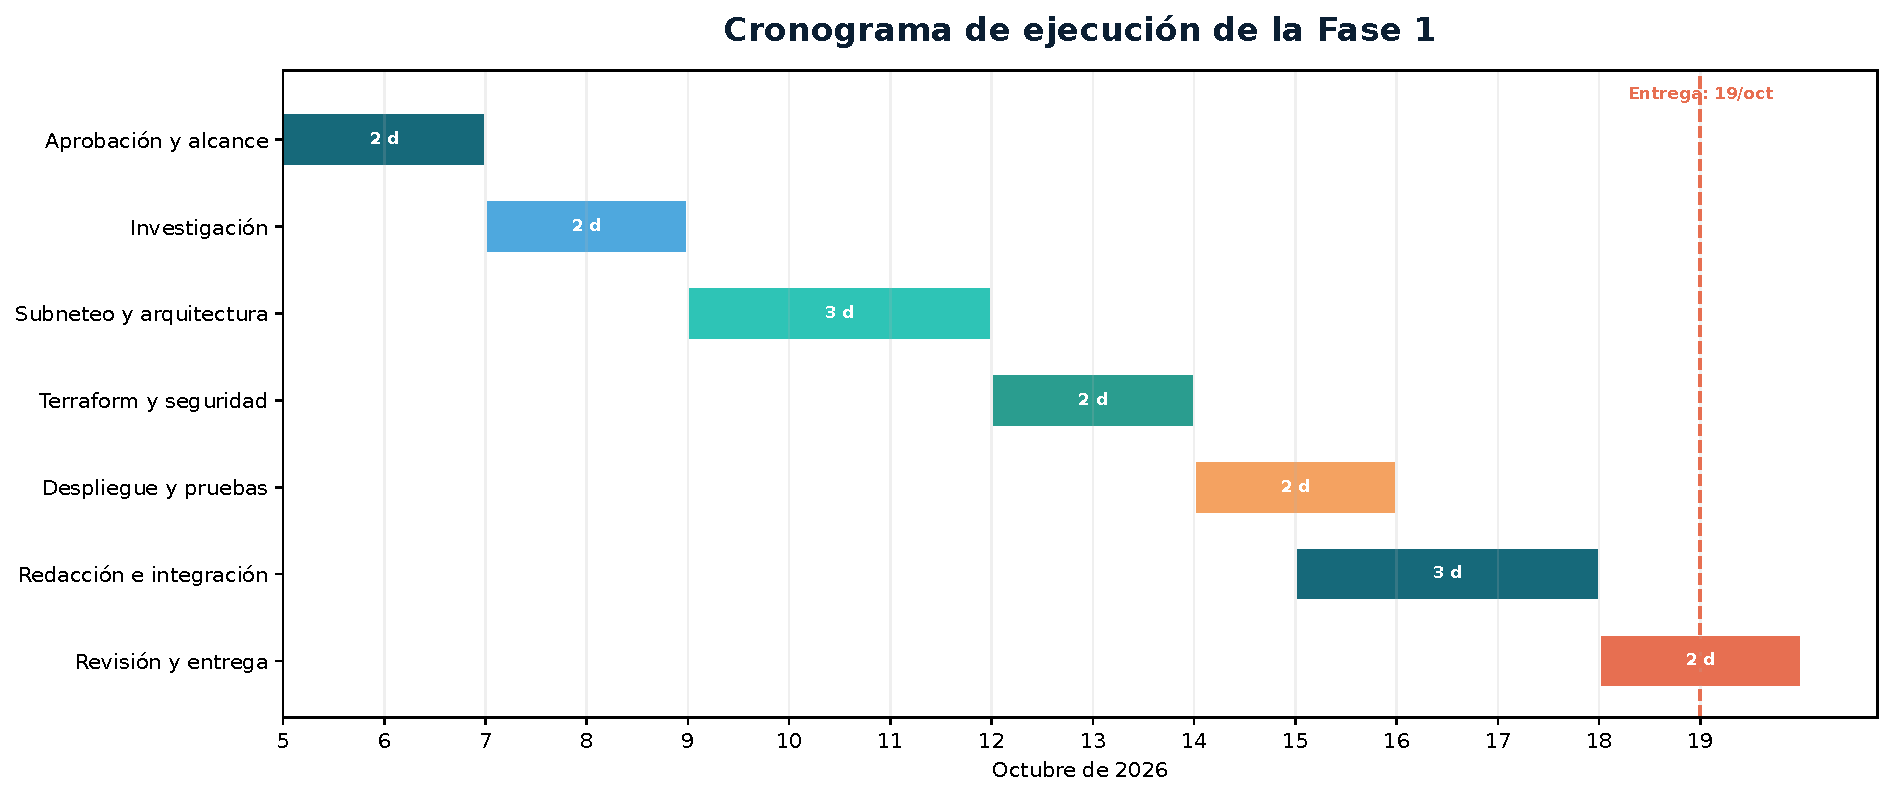
\includegraphics[width=\textwidth]{cronograma.pdf}
\caption{Cronograma de la Fase 1. Elaboración propia.}
\label{fig:gantt}
\end{figure}

\section{Responsabilidades}

\begin{table}[H]
\centering
\caption{Distribución propuesta de responsabilidades}
\begin{tabularx}{\textwidth}{p{4.5cm}Y Y}
\toprule
\textbf{Integrante} & \textbf{Responsabilidad principal} & \textbf{Revisión cruzada} \\
\midrule
Pablo Daniel Barillas Moreno & Coordinación, integración LaTeX, repositorio y compilación final. & Implementación y evidencias. \\
Andrés Rafael Chivalán & Cálculos de subneteo, arquitectura y consistencia de diagramas. & Revisión matemática y narrativa. \\
Roberto Emiliano Otoniel Camposeco Torres & Terraform, ejecución AWS, pruebas y destrucción. & Seguridad y anexos técnicos. \\
\bottomrule
\end{tabularx}
\end{table}

La asignación no elimina la responsabilidad conjunta. Toda modificación de direccionamiento debe ser revisada por otra persona; todo despliegue requiere confirmación del responsable de costos; y el PDF final debe ser leído por al menos dos integrantes.

\section{Hitos y puertas de calidad}

\begin{longtable}{p{2.2cm}p{4.1cm}p{7.1cm}}
\toprule
\textbf{Hito} & \textbf{Salida} & \textbf{Puerta de calidad} \\
\midrule
\endfirsthead
\toprule
\textbf{Hito} & \textbf{Salida} & \textbf{Puerta de calidad} \\
\midrule
\endhead
H1 & Alcance y supuestos & Cantidad de Visitas y composición del equipo visibles. \\
H2 & Selección de proveedor & Matriz ponderada, fuentes oficiales y decisión explicada. \\
H3 & Plan CIDR & Fórmulas, máscaras, reservas, rangos y script coinciden. \\
H4 & Código Terraform & Formato y validación sin errores; secretos excluidos. \\
H5 & Despliegue & Cuenta, región, costo y recursos identificados. \\
H6 & Pruebas & Ping real, prueba negativa y evidencia con fecha. \\
H7 & Cierre & Destrucción confirmada, PDF revisado y repositorio limpio. \\
\bottomrule
\end{longtable}

\section{Registro de riesgos}

\begin{longtable}{p{3.7cm}C{1.6cm}C{1.6cm}p{6.2cm}}
\toprule
\textbf{Riesgo} & \textbf{Prob.} & \textbf{Impacto} & \textbf{Respuesta} \\
\midrule
\endfirsthead
\toprule
\textbf{Riesgo} & \textbf{Prob.} & \textbf{Impacto} & \textbf{Respuesta} \\
\midrule
\endhead
Credenciales AWS ausentes & Alta & Alto & Configurar una identidad autorizada localmente; nunca copiar claves al informe o Git. \\
Permisos insuficientes & Media & Alto & Revisar errores por acción y ajustar sólo los permisos necesarios. \\
Cargos imprevistos & Media & Alto & Cómputo apagado por defecto, sin NAT, ventana corta y destrucción obligatoria. \\
CIDR incorrecto & Baja & Alto & Script de contención y no solapamiento antes de planificar. \\
SSH inaccesible & Media & Medio & Confirmar IP \code{/32}, reglas, llave y estado antes de probar. \\
ICMP bloqueado & Media & Medio & Verificar pertenencia al mismo SG y usar IP privada correcta. \\
Capturas ilegibles & Media & Medio & Recortar al recurso relevante y acompañar con pie explicativo. \\
PDF con desbordes & Baja & Medio & Renderizar todas las páginas e inspeccionar tablas y figuras. \\
Secreto en Git & Baja & Crítico & Revisar \code{git diff}, patrones de exclusión y escaneo textual antes del push. \\
\bottomrule
\end{longtable}

\section{Definición de terminado}

La fase se considera completa únicamente cuando: los requisitos tienen trazabilidad; los cálculos son reproducibles; Terraform valida; la infraestructura se despliega en una cuenta autorizada; el ping y el aislamiento producen evidencia; los recursos se destruyen; el PDF no presenta defectos; y el repositorio remoto contiene todos los entregables sin secretos. Si falta una condición, su estado se declara explícitamente.
